\documentclass[11pt]{article}
\usepackage[a4paper,margin=1in]{geometry}
\usepackage{amsmath,amssymb,amsthm,mathtools}
\usepackage{booktabs}
\usepackage{enumitem}
\usepackage{graphicx}
\usepackage{microtype}
\usepackage{hyperref}
\usepackage[nameinlink,capitalise]{cleveref}
\usepackage[numbers,sort&compress]{natbib}

\newtheorem{theorem}{Theorem}[section]
\newtheorem{proposition}[theorem]{Proposition}
\newtheorem{corollary}[theorem]{Corollary}
\newtheorem{lemma}[theorem]{Lemma}
\theoremstyle{definition}
\newtheorem{definition}[theorem]{Definition}
\theoremstyle{remark}
\newtheorem{remark}[theorem]{Remark}
\newcommand{\norm}[1]{\left\lVert#1\right\rVert}
\newcommand{\tr}{\operatorname{tr}}
\newcommand{\Ran}{\operatorname{Ran}}
\newcommand{\E}{\mathcal E}

\title{Source-Seeded Four-Direction Horizon Refresh\\
\large Removing the Late Ambient Seed}
\author{Liang Wang}
\date{July 2026}

\begin{document}
\maketitle

\begin{abstract}
The recursive packet chain of RH-93 removes ambient eigenspace resets inside
one four-step block, but still starts that block from a late ambient leading
packet.  We move the only spectral seed to time zero and ask whether a
low-dimensional Ritz chain can carry it through the complete frozen prefix.

If $S$ is the source matrix, the initial normalized memory Gramian is
\[
 G_0=\frac{S^*S}{\norm{S}_F^2}.
\]
Its leading rank-$r$ packet is exactly the leading right singular subspace of
$S$.  Starting from this source packet, let $V_{t-1}$ be the current packet,
select $k$ left singular directions of
\[
 K_t=(I-V_{t-1}V_{t-1}^*)G_tV_{t-1},
\]
and retain the leading $r$ Ritz directions in the resulting
$(r+k)$-dimensional space.  We prove a source-seeded recursive horizon theorem:
every update preserves rank, improves the new-Gram predictor tail, and uses no
ambient leading eigenspace after time zero.  The exact gain remains
certifiable by a generalized bottom frame of the compressed matrix.

A 384-bit audit follows ten channels from the source to the RH-93 endpoint,
for a total of 120 primary updates.  Width two has worst endpoint/reference
tail ratio $11.397994$, and width three has worst ratio $1.448940$.  Width four
passes all ten endpoint gates, with worst ratio $1.001173$, minimum
projected-cross energy capture $97.536\%$, and compressed dimension at most
$11$.  All 120 direct Ritz updates are monotone and all generalized frame
gains are strictly positive.  The source-SVD and initial-Gram projectors agree
to at most $7.96\times10^{-14}$ in operator norm.

Thus the late ambient seed can be removed on the archived horizons.  The
initial source-coordinate SVD, the ambient action $G_tV_{t-1}$, repeated
all-level contraction, and continuum complexity bounds remain open.  No
Hilbert--Polya operator, zeta-zero identification, or Riemann Hypothesis
result is claimed.
\end{abstract}

\noindent\textbf{Keywords:} source Gramian; recursive Ritz method; projected
cross operator; low-rank packet; validated numerics.

\medskip
\noindent\textbf{MSC 2020:} 47A75; 15A18; 65F15; 65G20; 37C30.

\section{Introduction}

The late-memory route developed in the preceding layers seeks a
finite-dimensional packet that captures the dynamically relevant part of a
time-ordered Gramian.  The rank clock of RH-82 suggests
$r=O(\log(1/\sigma))$ at the archived scales \citep{WangRankClock2026}.
RH-92 replaced a rigid pointwise contraction target by a four-step product
budget \citep{WangBlockBudget2026}.  RH-93 then showed that two
projected-cross directions are enough to propagate the corrected packet
recursively inside each selected four-step block
\citep{WangRecursiveRitz2026}.

That result still left one visible ambient operation.  At the beginning of
each late block, the seed packet was obtained from the leading eigenspace of
the ambient Gramian.  The reduced recursion began only after that reset.  Such
a finite construction is mathematically legitimate, but it cannot yet serve
as an intrinsic all-prefix packet law.

The present paper asks the next minimal question:
\begin{quote}
Can the packet be seeded once from the source at time zero and then carried
recursively to the late endpoint without inserting any later ambient leading
eigenspace?
\end{quote}
There is a canonical seed.  At time zero the state is the source $S$, so the
normalized snapshot Gramian is $S^*S/\norm S_F^2$.  Its leading eigenspace is
the leading right singular subspace of $S$.  This observation is elementary,
but it changes the architecture of the certificate: the seed is now attached
to the input data rather than to a late dynamically assembled Gramian.

The algebraic part of the paper has two components.  First, we record the
source-seed equivalence with the correct spectral-gap qualification.  Second,
we formulate a recursive horizon theorem for an arbitrary finite sequence of
positive semidefinite Gramians.  It separates three operations:
\begin{enumerate}[leftmargin=2em]
\item apply the current Gramian to the incoming rank-$r$ packet;
\item identify $k$ projected-cross directions;
\item solve one $(r+k)$-dimensional Ritz problem.
\end{enumerate}
No ambient leading eigenspace occurs after initialization.  This is an exact
finite-dimensional statement, independent of the numerical model.

The numerical question is not whether the recursion exists, but how wide the
complement must be to retain endpoint accuracy over the complete prefix.  The
answer differs from the four-step contraction threshold.  Two directions were
enough locally in RH-93.  Over the source-to-endpoint horizon, width two can
lose more than a factor eleven relative to the ambient reference tail, and
width three can lose a factor $1.45$.  Width four is the first tested width
that is uniformly near the reference at all ten anchors.

This distinction is useful.  A narrow packet can satisfy a selected
contraction budget without identifying the leading packet accurately over a
long prefix.  Local contraction and horizon tracking are related but not
identical route gates.

\section{The source packet}
\label{sec:source}

Let $S:\mathbb C^m\to\mathbb C^n$ be nonzero.  We regard its columns as source
coordinates and define
\begin{equation}
 G_0=\frac{S^*S}{\norm S_F^2}.
 \label{eq:g0}
\end{equation}
Then $G_0=G_0^*\ge0$ and $\tr G_0=1$.

\begin{theorem}[Source-seed equivalence]
\label{thm:source-seed}
Let
\[
 S=U\Sigma Z^*
\]
be a singular-value decomposition with singular values in nonincreasing
order.  For every rank $r$, the span of the first $r$ columns of $Z$ is a
leading rank-$r$ eigenspace of $G_0$.  If
$s_r(S)>s_{r+1}(S)$, this rank-$r$ spectral subspace is unique.  Without a
gap, the two constructions determine the same family of admissible leading
subspaces.
\end{theorem}

\begin{proof}
Equation \eqref{eq:g0} gives
\[
 G_0=Z\frac{\Sigma^*\Sigma}{\norm S_F^2}Z^*.
\]
Thus the eigenvalues of $G_0$ are the squared singular values of $S$, divided
by their sum, and the corresponding eigenvectors are the right singular
vectors.  A strict cutoff gap gives uniqueness of the spectral projector.
When the cutoff is repeated, any rank-$r$ choice within the tied eigenspace is
simultaneously a leading right singular and a leading Gram eigenspace.
\end{proof}

\begin{remark}
The theorem does not eliminate a source-coordinate spectral operation.  It
identifies that operation intrinsically and places it at time zero.  Replacing
the source SVD by an analytic or structured seed construction is a later
problem.
\end{remark}

For the frozen model, let $X_t=T^tS$ and define the memory Gramians
\begin{equation}
 G_t=\frac{X_t^*X_t}{\tr(X_t^*X_t)}+\eta G_{t-1},
 \qquad \eta=\frac1{512},
 \qquad t\ge1.
 \label{eq:memory}
\end{equation}
The theorem applies because the recursion starts with \eqref{eq:g0}.  The
particular formula \eqref{eq:memory} is used only in the audit; the recursive
Ritz theorem below allows any finite positive semidefinite sequence.

\section{Source-seeded recursive horizon theorem}
\label{sec:horizon}

Let $G_0,\ldots,G_N$ be positive semidefinite matrices on a finite-dimensional
Hilbert space $\mathcal K$.  Let $V_0:\mathbb C^r\to\mathcal K$ be an
isometry spanning a leading rank-$r$ eigenspace of $G_0$.  Suppose
$V_{t-1}$ has already been constructed.  Put
\begin{equation}
 P_{t-1}=V_{t-1}V_{t-1}^*,
 \qquad
 K_t=(I-P_{t-1})G_tV_{t-1}.
 \label{eq:kt}
\end{equation}
Choose an isometry $Q_t:\mathbb C^k\to\Ran(I-P_{t-1})$ spanning the first
$k$ left singular directions of $K_t$, omitting zero directions if the cross
rank is smaller.  Set $Z_t=[V_{t-1},Q_t]$ and
\begin{equation}
 H_t=Z_t^*G_tZ_t
 =\begin{pmatrix}A_t&B_t\\B_t^*&D_t\end{pmatrix}.
 \label{eq:ht}
\end{equation}
Let $C_t$ contain the leading $r$ orthonormal eigenvectors of $H_t$ and define
\begin{equation}
 V_t=Z_tC_t.
 \label{eq:vt}
\end{equation}

For an isometric packet $V$, write
\[
 \E_G(V)=\tr G-\tr(V^*GV).
\]

\begin{theorem}[Source-seeded recursive horizon theorem]
\label{thm:horizon}
The recursion \eqref{eq:kt}--\eqref{eq:vt} has the following properties.
\begin{enumerate}[leftmargin=2em]
\item Every $V_t$ is an isometry of rank $r$ and is constructed in a space of
dimension at most $r+k$.
\item At every update,
\begin{equation}
 \E_{G_t}(V_t)\le \E_{G_t}(V_{t-1}).
 \label{eq:predictor-monotone}
\end{equation}
\item If the eigenvalues of $H_t$ are written in increasing order, the exact
captured-energy gain is
\begin{equation}
 \Delta_t
 =\tr D_t-\sum_{j=1}^k\lambda_j^\uparrow(H_t)\ge0.
 \label{eq:gain}
\end{equation}
\item After $V_0$ is chosen, no leading eigenspace of an ambient $G_t$ is
needed anywhere in the recursion.
\end{enumerate}
\end{theorem}

\begin{proof}
The columns of $Z_t$ are orthonormal, so \eqref{eq:vt} is an isometry with
$r$ columns.  Its range lies in $\Ran Z_t$, whose dimension is at most
$r+k$.

The old coordinate packet $V_{t-1}=Z_t[I_r,0]^T$ is an admissible rank-$r$
trial subspace in $\Ran Z_t$.  Ky Fan's maximum principle therefore implies
that the leading rank-$r$ Ritz packet captures at least as much $G_t$-energy
as $V_{t-1}$, proving \eqref{eq:predictor-monotone}
\citep{Fan1949,Bhatia1997}.  The sum of the leading $r$ eigenvalues of $H_t$
is
\[
 \tr H_t-\sum_{j=1}^k\lambda_j^\uparrow(H_t).
\]
Subtracting the old capture $\tr A_t$ and using
$\tr H_t=\tr A_t+\tr D_t$ gives \eqref{eq:gain}.  Finally,
\eqref{eq:kt} requires $G_tV_{t-1}$, and \eqref{eq:vt} requires only the
compressed eigensolve for $H_t$.  Neither operation asks for a leading
eigenspace of $G_t$.
\end{proof}

\begin{remark}[Meaning of ambient-free seed]
The late ambient \emph{eigenspace} seed is removed.  The matrix action
$G_tV_{t-1}$ remains ambient.  This distinction is essential: the theorem is
a low-dimensional spectral reduction, not yet a continuum complexity result.
\end{remark}

\subsection{Projected-cross selection}

The projected cross operator has only $r$ columns.  Its selected directions
maximize captured cross Frobenius energy:
\begin{equation}
 \max_{\substack{Q^*Q=I_k\\Q^*V=0}}
 \norm{Q^*GV}_{S_2}^2
 =\sum_{j=1}^k s_j\big((I-VV^*)GV\big)^2.
 \label{eq:cross-max}
\end{equation}
This is the Ky Fan principle applied to $KK^*$, or equivalently the
Eckart--Young singular-subspace characterization
\citep{GolubVanLoan2013}.  The unselected cross energy is
\begin{equation}
 \norm{(I-QQ^*)K}_{S_2}^2=\sum_{j>k}s_j(K)^2.
 \label{eq:cross-tail}
\end{equation}

One useful reduced identity is already visible:
\begin{equation}
 K^*K
 =V^*G(I-VV^*)GV
 =V^*G^2V-(V^*GV)^2.
 \label{eq:reduced-cross-gram}
\end{equation}
Thus the cross singular values and right singular vectors are determined by
an $r\times r$ positive semidefinite matrix.  Turning
\eqref{eq:reduced-cross-gram} into a complete stable factorization, including
small-singular-value thresholds and reconstruction of the left directions,
is the natural next layer.

\subsection{Generalized bottom-frame certificate}

For a full-column-rank frame
$W\in\mathbb C^{(r+k)\times k}$ define
\[
 \mathcal R_{H_t}(W)
 =\tr\!\left((W^*W)^{-1}W^*H_tW\right).
\]
Ky Fan's minimum principle gives
\[
 \sum_{j=1}^k\lambda_j^\uparrow(H_t)
 \le \mathcal R_{H_t}(W).
\]
Consequently
\begin{equation}
 \tr D_t-\mathcal R_{H_t}(W)>0
 \quad\Longrightarrow\quad
 \Delta_t>0.
 \label{eq:frame}
\end{equation}
The generalized form is invariant under a nonsingular change of frame
coordinates and is therefore appropriate for outward-rounded verification.

\section{Validated experiment}
\label{sec:audit}

\subsection{Frozen protocol}

We use the same five noise scales, two directional channels, normalized
memory parameter, and half-log rank clock as RH-82--RH-93.  The scales are
\[
 \sigma\in\{0.16,0.08,0.04,0.02,0.01\}.
\]
For inherited horizons $4,9,16,25,32$, respectively, the late endpoints are
\[
 N_\sigma=\max\{4,\lceil 2H_\sigma/3\rceil\}
 \in\{4,6,11,17,22\}.
\]
Each channel begins from the leading right singular packet of its source.
The complete chain from $t=1$ through $N_\sigma$ is then run independently
at widths two, three, and four.

All source matrices, Gramians, packets, compressed frames, and reported tail
forms are interpreted as exact binary inputs to Arb at 384-bit precision.
Outward endpoints are used for every inequality.  The SVD, QR factorization,
and symmetric eigensolves select trial subspaces in double precision; Arb
then certifies the claimed quadratic forms for those concrete subspaces.
This is a standard validated-numerics division of labor
\citep{Higham2002,Rump2010}.

The primary width-four audit contains
\[
 2(4+6+11+17+22)=120
\]
updates.  At every update we record the predictor tail, corrected tail,
ambient reference tail, generalized frame gain, frame metric determinant,
cross-energy fraction, and orthogonality defects.

\subsection{Endpoint width threshold}

\begin{table}[t]
\centering
\caption{Outward upper bounds for endpoint tail divided by the ambient
leading-packet tail.  Width four passes the $1.01$ gate in all channels.}
\label{tab:endpoints}
\begin{tabular}{@{}lrrr@{}}
\toprule
channel & width 2 & width 3 & width 4\\
\midrule
$0.16$ left  & 1.000004 & 1.000001 & 1.000001\\
$0.16$ right & 1.232685 & 1.000006 & 1.000007\\
$0.08$ left  & 1.163776 & 1.000500 & 1.000001\\
$0.08$ right & 11.397994 & 1.021816 & 1.000001\\
$0.04$ left  & 2.778159 & 1.004185 & 1.000001\\
$0.04$ right & 6.891207 & 1.448940 & 1.000001\\
$0.02$ left  & 1.033230 & 1.003791 & 1.000003\\
$0.02$ right & 3.623212 & 1.143370 & 1.000002\\
$0.01$ left  & 1.025773 & 1.000862 & 1.000006\\
$0.01$ right & 5.939843 & 1.014986 & 1.001173\\
\bottomrule
\end{tabular}
\end{table}

\Cref{tab:endpoints} gives the central finite result.  Width two is not a
robust horizon-tracking law, despite its success on the selected late
four-step contraction windows.  Width three substantially improves the
chain, but one channel still reaches $1.448940$.  Width four remains within
$0.118\%$ of the reference in every channel.

This is not a theorem that four directions are universally minimal.  It is a
sharp threshold among the three archived constructions at the fixed rank
clock and frozen horizons.  In particular, recursive chains of different
widths diverge after their first update, so one cannot compare their endpoints
by a simple nesting argument.

\subsection{Mechanism diagnostics}

The minimum selected projected-cross energy fractions over all updates are
\[
 0.7949096\quad(k=2),\qquad
 0.8945814\quad(k=3),\qquad
 0.9753653\quad(k=4).
\]
The fourth direction therefore removes most of the residual cross tail left
by width three.  This diagnostic is consistent with the endpoint transition,
although \eqref{eq:cross-tail} alone does not control the Ritz tail: the
complement diagonal block and joint rotation also matter.

All 120 width-four corrected tails are no larger than their incoming
predictor tails.  Every generalized frame gain in \eqref{eq:frame} is
strictly positive; the smallest validated lower bound is
$2.16\times10^{-14}$.  The smallest frame metric determinant is larger than
$0.999999999999996$, and the largest orthogonality defect is below
$2.74\times10^{-15}$.  The compressed dimension is at most $r+4=11$.

The source seed was also computed independently from the source SVD and from
the leading eigenspace of $G_0$.  The largest operator-norm distance between
the two numerical projectors is $7.96\times10^{-14}$, in agreement with
\cref{thm:source-seed}.

The endpoint result should not be confused with pointwise reference
tracking.  The largest intermediate width-four tail/reference ratio is
$3.023179$.  The recursive packet may temporarily depart from the ambient
leading packet and recover later.  The theorem guarantees predictor
improvement, while the audit certifies endpoint recovery.

\begin{figure}[t]
\centering
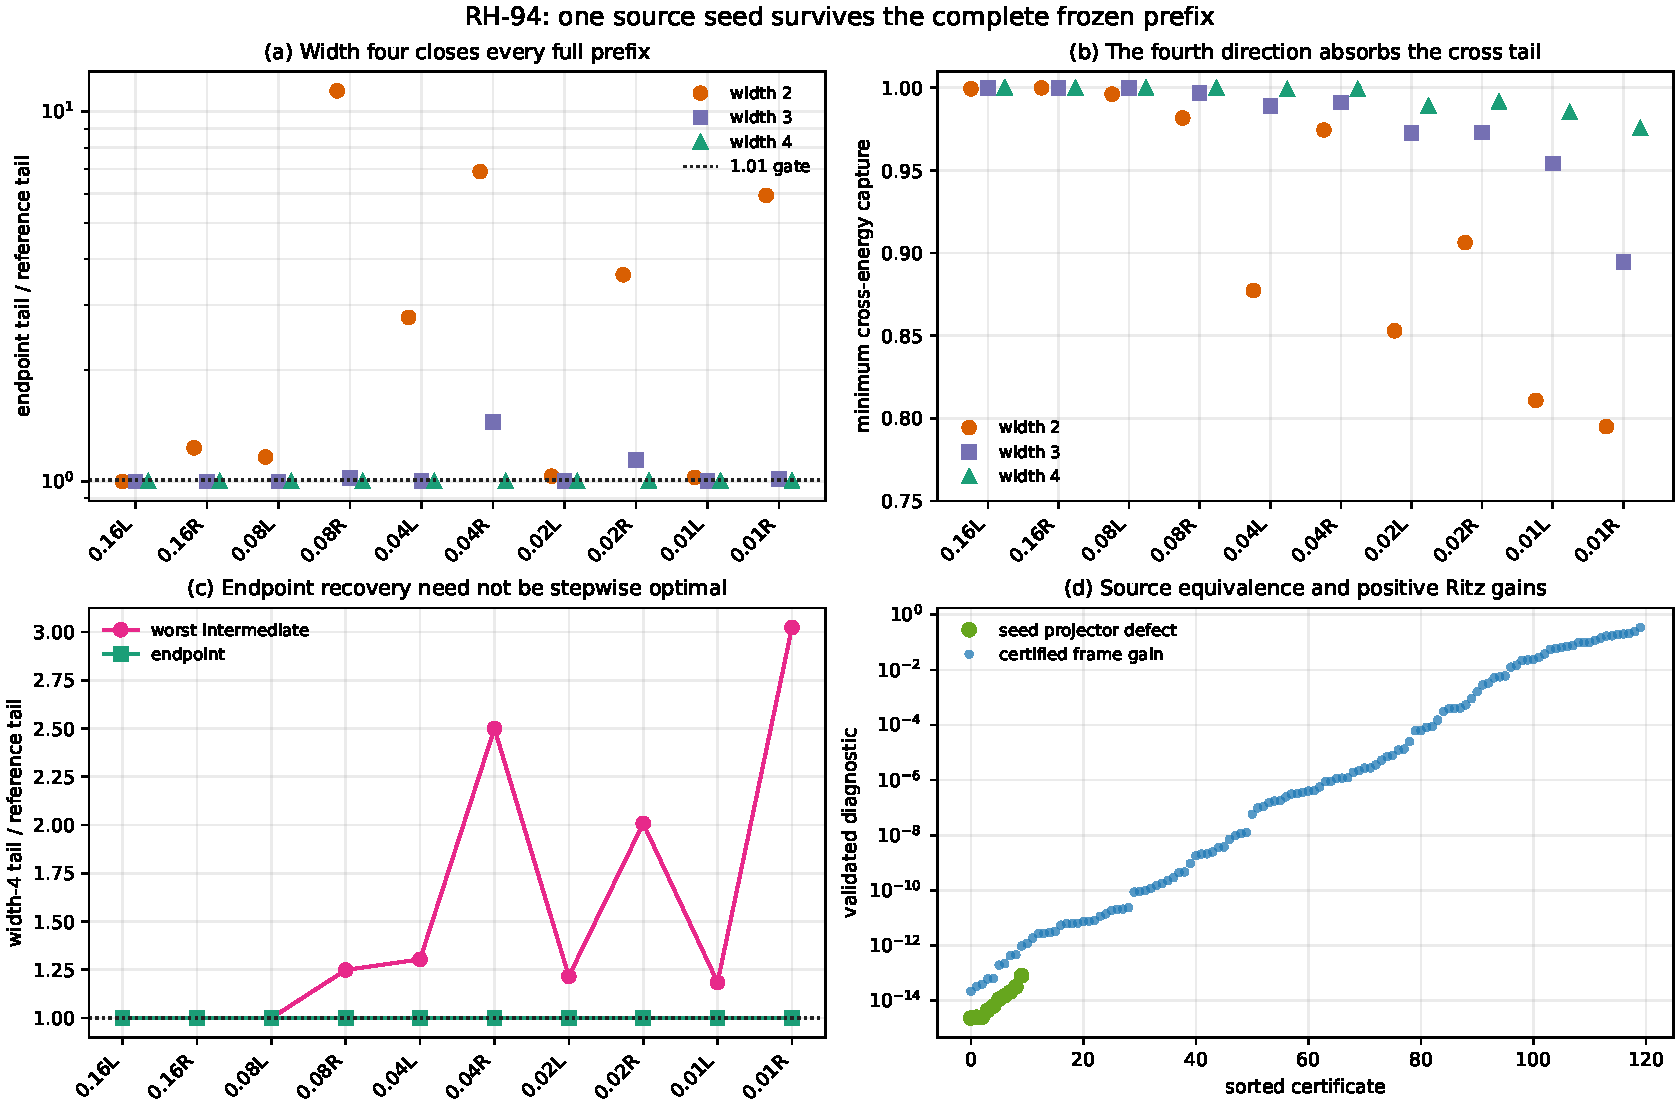
\includegraphics[width=\textwidth]{figures/source_seeded_four_direction_horizon.pdf}
\caption{Full-prefix source-seeded refresh.  Width four closes all endpoint
gates, captures at least $97.536\%$ of projected-cross energy, and recovers at
the endpoint even when intermediate reference ratios are larger.}
\label{fig:audit}
\end{figure}

\section{Consequences for the route}
\label{sec:route}

RH-94 changes the finite architecture in one precise way.  A late ambient
leading eigenspace is no longer needed to start the reduced recursion.  The
entire frozen prefix can be represented as
\[
 \text{source packet}
 \longrightarrow
 \text{projected-cross action}
 \longrightarrow
 \text{small Ritz refresh}
 \longrightarrow\cdots\longrightarrow
 \text{late endpoint}.
\]

It is useful to keep two width statements separate:
\begin{itemize}[leftmargin=2em]
\item \emph{two-direction block law}: sufficient for the RH-93 four-step
contraction target on the selected late windows;
\item \emph{four-direction horizon law}: sufficient for near-reference
source-to-endpoint tracking on all ten frozen channels.
\end{itemize}
The first is economical for contraction.  The second is stronger for packet
identification.  A future proof may use the width-four chain during burn-in
and switch to width two inside a stable repeated-block regime.

The next obstruction is also clearer.  Equation
\eqref{eq:reduced-cross-gram} reduces direction \emph{selection} to an
$r\times r$ matrix, but constructing the left directions still uses
$G_tV_{t-1}$.  A reduced factorization should:
\begin{enumerate}[leftmargin=2em]
\item diagonalize $K_t^*K_t$ rather than an ambient cross matrix;
\item reconstruct only directions whose singular values exceed a certified
threshold;
\item quantify how discarded cross singular values perturb the corrected
tail;
\item state exactly which moments $V^*G^jV$ and ambient packet actions remain.
\end{enumerate}
That is a bounded and testable next problem, rather than an appeal to an
unspecified continuum limit.

\section{Claim boundary}

The present result is deliberately finite.
\begin{enumerate}[leftmargin=2em]
\item The source SVD is an initial source-coordinate spectral operation.  It
has been identified, not eliminated.
\item Applying $G_t$ to a rank-$r$ packet remains an ambient operation.  The
spectral solve is reduced, but a continuum complexity theorem is absent.
\item Only five frozen scales and two channels are audited.  No uniform
all-level width-four theorem follows from ten anchors.
\item Endpoint recovery does not imply stepwise closeness to the ambient
leading packet.
\item No repeated-block contraction theorem, normalization/observability
bridge, moving-cloud trace-class limit, Hilbert--Polya operator, zeta-zero
identification, or proof of the Riemann Hypothesis is obtained.
\end{enumerate}

\section{Conclusion}

The late ambient seed in the recursive packet route is not structurally
necessary on the archived horizons.  The leading source right singular
subspace is exactly the initial Gram packet, and four projected-cross
directions carry that packet through all 120 updates with near-reference
endpoint tails.  Widths two and three do not provide the same robust horizon
tracking, so the full-prefix problem reveals a new finite width threshold not
visible in the late four-step contraction test.

The route now begins at a genuine source object and remains recursively
low-dimensional in its spectral solves.  Its next mathematical task is the
projected-cross Gram reduction \eqref{eq:reduced-cross-gram}: turn the ambient
cross SVD into a stable small-matrix factorization and derive a quantitative
tail criterion for discarded directions.

\bibliographystyle{plainnat}
\bibliography{references}

\end{document}
